\section{Experimental Evaluation}
\label{sec:experiments}
To understand the trade-offs between these Distribution Strategies (DSs), we perform four sets of experiments using queries over target families presented on the GtoPdb website. The first set of experiments use real queries extracted from citations to GtoPdb published in the British Journal of Pharmacology.  
The second set uses synthetically produced provenance polynomials, corresponding to more complex queries, in order to highlight the differences between the DSs.
The third set of experiments considers the accrual of credit over time by the three strategies, again using synthetic queries.
The fourth set of experiments shows how the DSs compare to traditional citations in giving credit to data curators using both real and synthetic queries. We close by discussing relative execution times of the three strategies.

\subsection{Real-world queries}
\label{sec:real_world_queries}

\begin{figure}[t]
  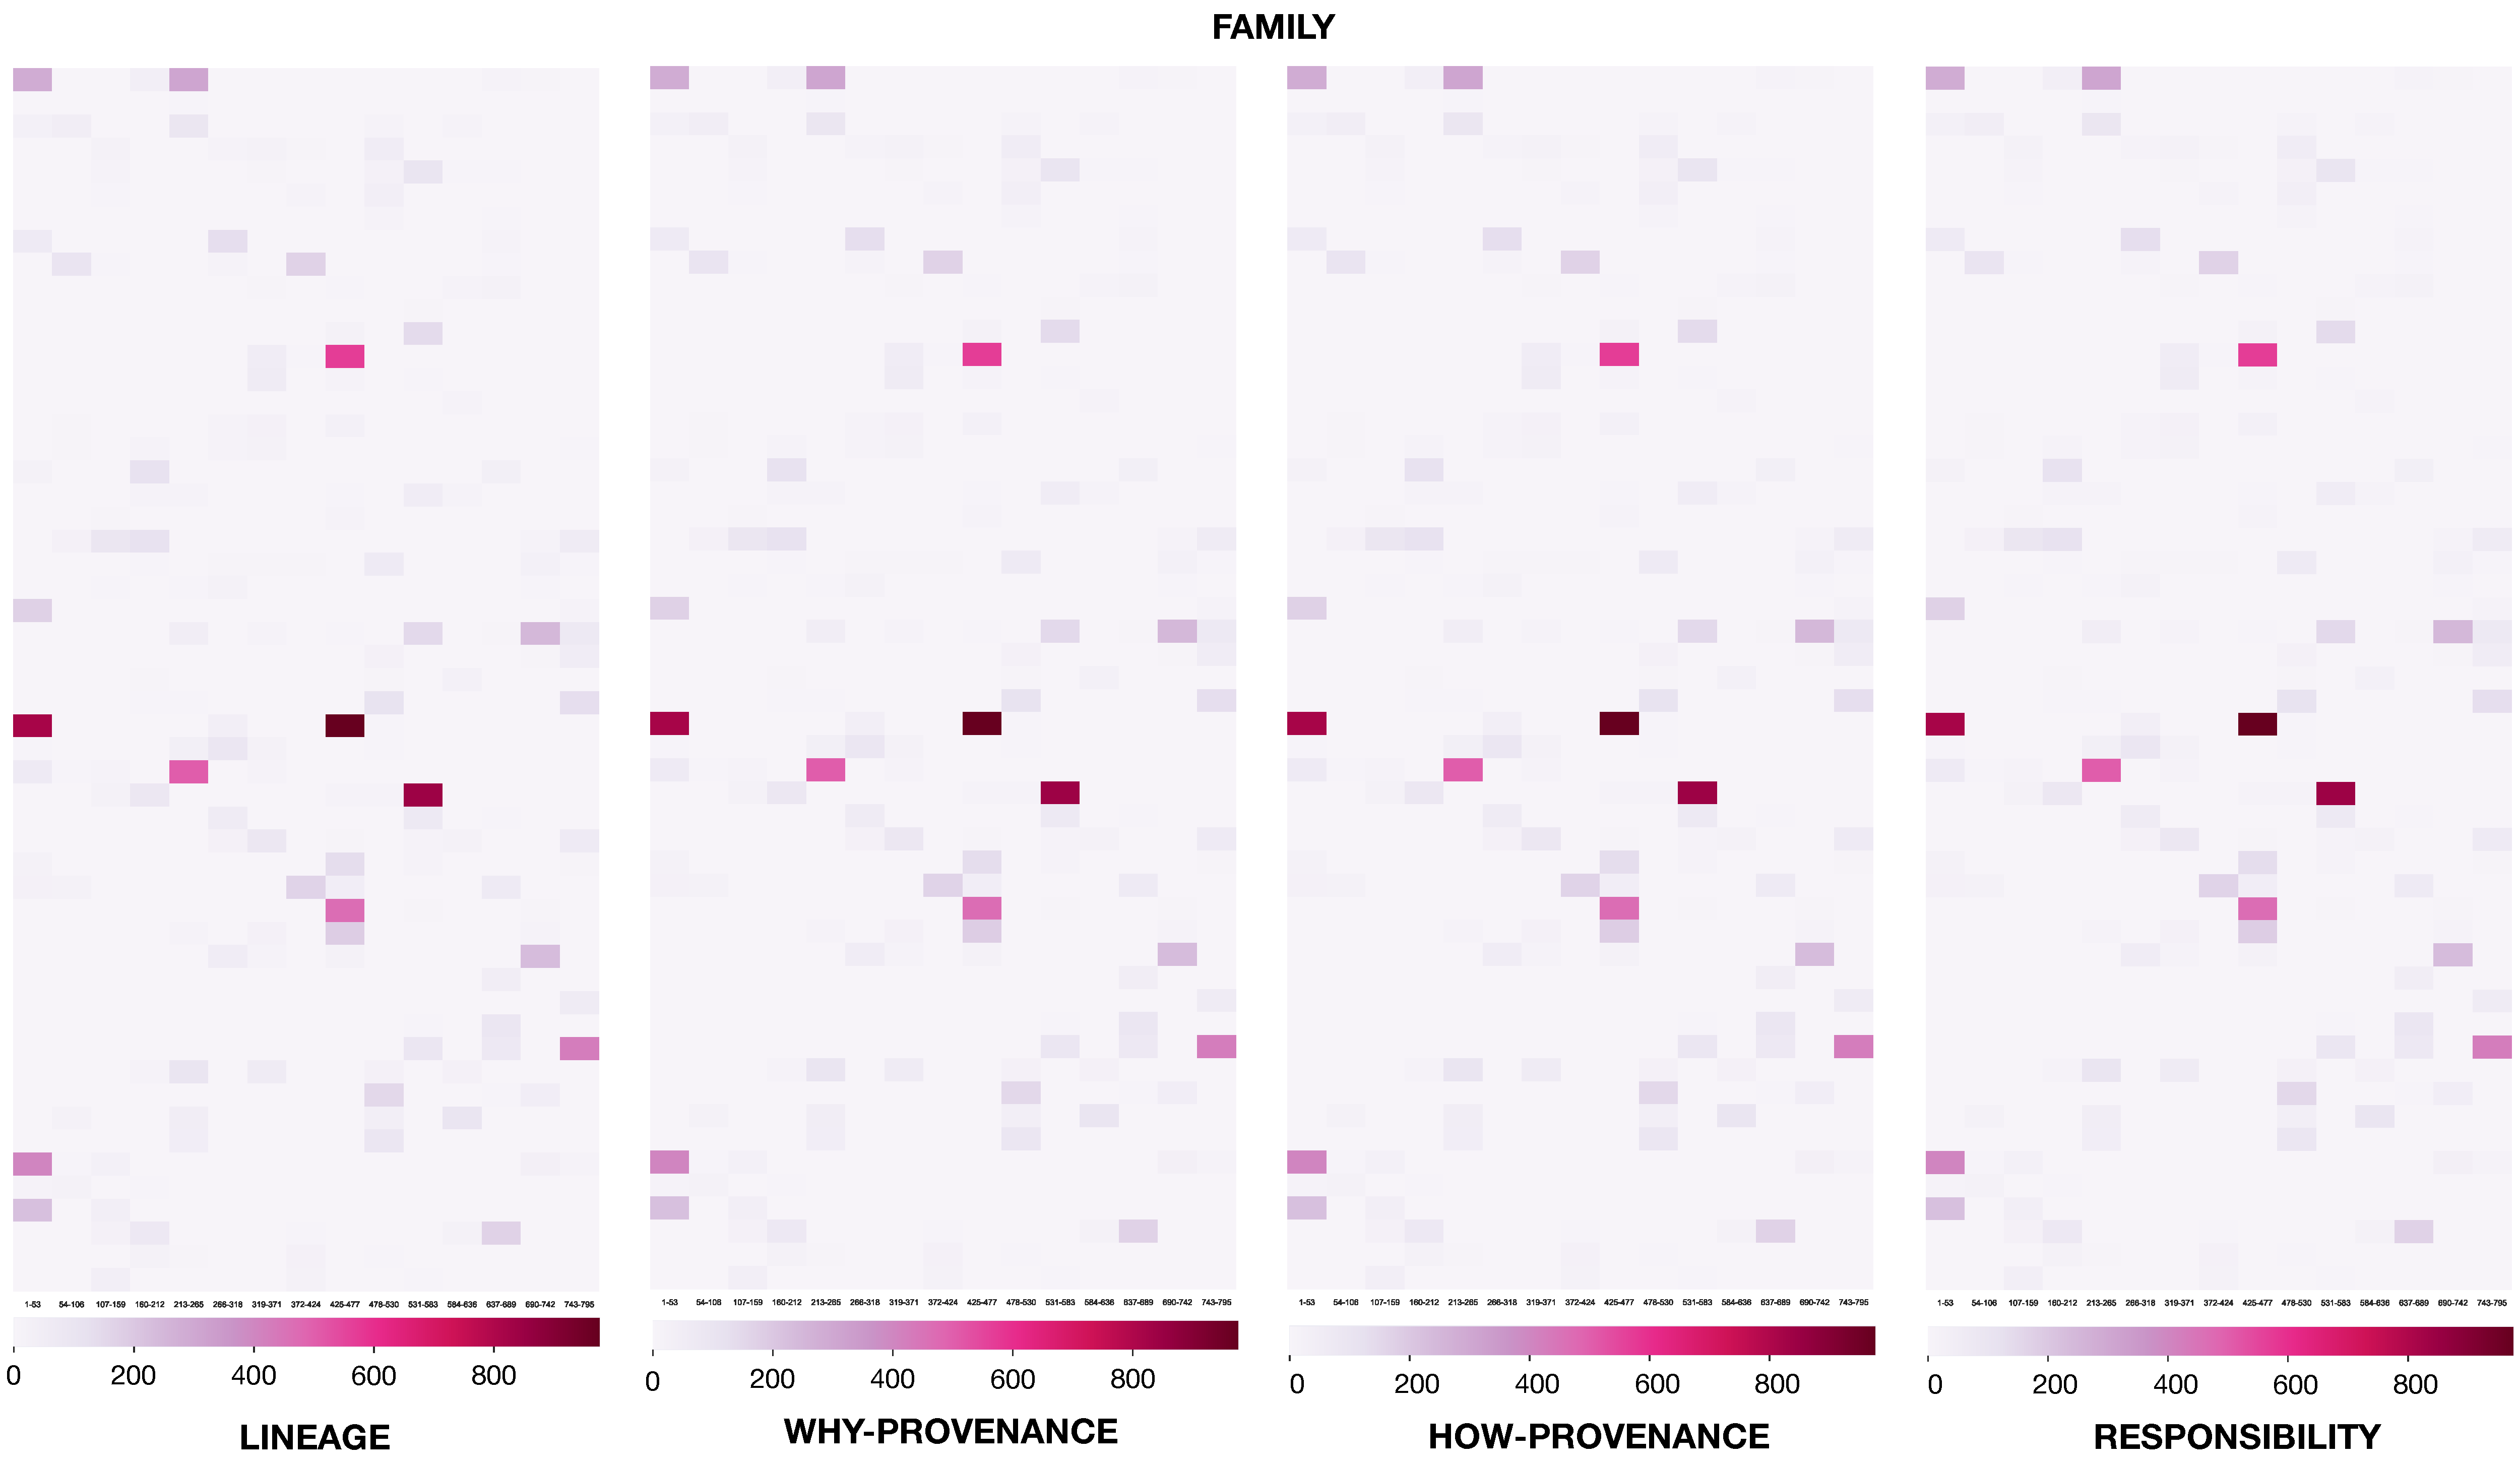
\includegraphics[width=1\textwidth]{figures/paper_based}
  \caption{Comparison of three DS on the same table \texttt{family} using the distribution given by the queries retrieved from papers.}
  \label{figure:comparison_on_papers}
\end{figure}


%We evaluate the proposed distribution strategies on GtoPdb, and in particular, we focus on target families described on the GtoPdb website. 

%When a paper uses data from GtoPdb, it can cite the full database, a webpage of interest, or a subset of data extracted with a query. 

Examples of real queries are drawn
from papers published in the British Journal of Pharmacology (BJP).~\footnote{\url{https://bpspubs.onlinelibrary.wiley.com}}  Each time a paper in this journal cites a webpage from GtoPdb, it reports the URL of the page. From this URL, the query used to obtain the webpage data can be determined. 
We considered all $889$ papers in BJCP citing the IUPHAR/BPS Guide to pharmacology \citep{iuphar2018} as of October 2020, and extracted all webpage URLs to GtoPdb contained within the paper\footnote{The IUPHAR/BPS Guide is a journal that describes the structure and evolution of GtoPdb. At the time of writing, it had received more than $1200$ citations on Google Scholar.}.
\scream{Revised, check that it is correct.}

%\eat{
There are eight target family types presented on the GtoPdb website: \emph{GPCR}, \emph{Ion channels}, \emph{NHRs}, \emph{Kinases}, \emph{Catalytic receptors}, \emph{Transporters}, \emph{Enzymes} and \emph{Other protein targets}.  
%}

The queries that we inferred are those used to build target family webpages.  An example was given in Figure \ref{figure:family_structure}, where we show how the structure of the ``Adenosine receptors'' family can be mapped into  queries over the underlying database. %to get the information reported in the corresponding webpage. 
In GtoPdb, all target family pages share a similar structure; the only difference is that individual sections, such as ``contributors'' or ``further readings'', may be absent.
Therefore, the same queries can be used to build all of the target family pages by simply changing the family id used in the query (in Figure \ref{figure:family_structure}, it is 3).
Note that the queries are fairly simple SQL queries, and fall into a class called ``select-project-join" or ``SPJ" queries. 
A total of more than $12K$ different queries were built in this way.\footnote{For reproducibility purposes, the code we used for our experiments and all queries are available here: \url{https://bitbucket.org/dennis_dosso/credit_distribution_project}.}
Without loss of generality, we give each tuple in the output of a query a credit of $1$.

\paragraph{Results} Figure \ref{figure:comparison_on_papers} shows the heat-maps obtained by the distribution of credit according to the three different DS on one of the tables in the underlying database, \texttt{family},
%describes the characteristics and necessary information of the receptor families and, as can be seen in Figure \ref{figure:family_structure}, it 
which is often joined with other tables in the database to build the webpages.
It can be seen that the result of  credit distribution over \texttt{family} is the same for all three strategies. The same result is also obtained with the other tables of the database used by the queries shown in Figure \ref{figure:family_structure}. 

The reason why credit distribution is the same for all three strategies is that the queries are all simple SPJ queries, which use each table only once and do joins on key attributes. 
Under these conditions, each tuple of the output presents: (i) a how-provenance that is a single monomial with coefficient $1$ and exponent $1$ in each variable; (ii) a why-provenance with only one witness; and (iii) a lineage that coincides with the witness in the basis.
Hence, for these queries, the three DSs behave in the same way:
Credit is uniformly distributed among the tuples present in each provenance. 

To illustrate this, consider one of the queries in Figure \ref{figure:family_structure} which is used to build the output webpage:

\vspace{2mm}
{\footnotesize
\begin{adjustwidth}{25pt}{5pt}
	\begin{verbatim}
	Q3: SELECT c.first_names, c.surname
	FROM contributor2family AS cf JOIN contributor AS c ON 
	cf.contributor_id = c.contributor_id 
	WHERE f.family_id = 3
\end{verbatim}
\end{adjustwidth}
}
\vspace{2mm}

\texttt{Q3} returned $10$ tuples from the version of GtoPdb used. 
The first tuple, \texttt{<Bertil B., Fredholm>}, has  $c_{939} \cdot c2f_{496}$ as its provenance polynomial.
$c_{939}$ represents the provenance token of a tuple in \texttt{contributor}, and $c2f_{496}$ the provenance token of a tuple in table \texttt{contributor2family}. 
The why-provenance of this tuple is $\{\{c_{939}, cf_{496} \}\}$ and its lineage is $\{c_{939}, c2f_{496} \}$.
Therefore, the credit assigned to these tuples is $1/2$ using all three DS.
This happens for all the tuples in the output of each query of GtoPdb, thus making the distributions equivalent over all outputs.

However, this is not the case with more complex queries. As we showed in the previous section, when two or more tuples are merged as a result of a projection or union, the credit distributions will differ between the three strategies. %These are represented as multiple witnesses and multiple monomials. 

\begin{comment}
	
To give an example of how the CDS can differ from one another in their behavior, let us consider a different query:

\vspace{2mm}
{\footnotesize
\begin{adjustwidth}{25pt}{5pt}
	\begin{verbatim}
	Q4: SELECT f.name AS name
	FROM family AS F JOIN
	(SELECT DISTINCT f.family_id, f.name
	FROM "family" AS f JOIN contributor2family AS cf ON 
	f.family_id = cf.family_id 
	JOIN contributor c ON 
	cf.contributor_id = c.contributor_id 
	WHERE c.country = 'UK') AS R 
	ON F.name = R.name
\end{verbatim}
\end{adjustwidth}
}
\vspace{2mm}

Here the innermost query retrieves all the names and ids of the families written by an author from the UK producing a relation called $R$. This relation is then joined with the table \texttt{family} on the attribute \texttt{name}. 

One output tuple of this query is \texttt{<Histamine receptors>}, that has the following provenance polynomial:

{\footnotesize
\[
\begin{array}{c}
	f_{625}(f_{625} c2f_{656} c_{184} + f_{625} c2f_{113} c_{180} + f_{625} c2f_{283} c_{198} +\\ 
	+ f_{625} c2f_{550} c_{865} + f_{625} c2f_{573} c_{101} + f_{625} c2f_{95} c_{109} )
\end{array}
\]
}

As already discussed, the different monomials represent possible \emph{alternatives} of combinations of tuples that produce the considered output tuple. 
Tuple $f_{625}$ is used multiple times with different joins, thus it appears in each monomial. 
The last join, performed in the outmost query, is responsible for the final multiplication of $f_{625}$ with the rest of the polynomial between parenthesis.

From this polynomial we compute the why-provenance as a set of six different witnesses:

{\footnotesize
\[
\begin{array}{c}
\{\{ f_{625}, c2f_{656}, c_{184} \}, \{ f_{625}, c2f_{113}, c_{180} \} 
\{ f_{625}, c2f_{283}, c_{198} \}, \\ \{ f_{625}, c2f_{550}, c_{865} \},
 \{ f_{625}, c2f_{573}, c_{101}\} , \{f_{625}, c2f_{95}, c_{109} \}\}	\\
\end{array}
\]
}

And corresponding lineage:
{\footnotesize
\[
\begin{array}{c}
	\{ f_{625}, c2f_{656}, c_{184}, c2f_{113}, c_{180}, 
  c2f_{283}, c_{198}, c2f_{550}, c_{865}, 
  c2f_{573}, c_{101}, c2f_{95}, c_{109}\}
\end{array}
\]
}

\begin{figure}[tb]
  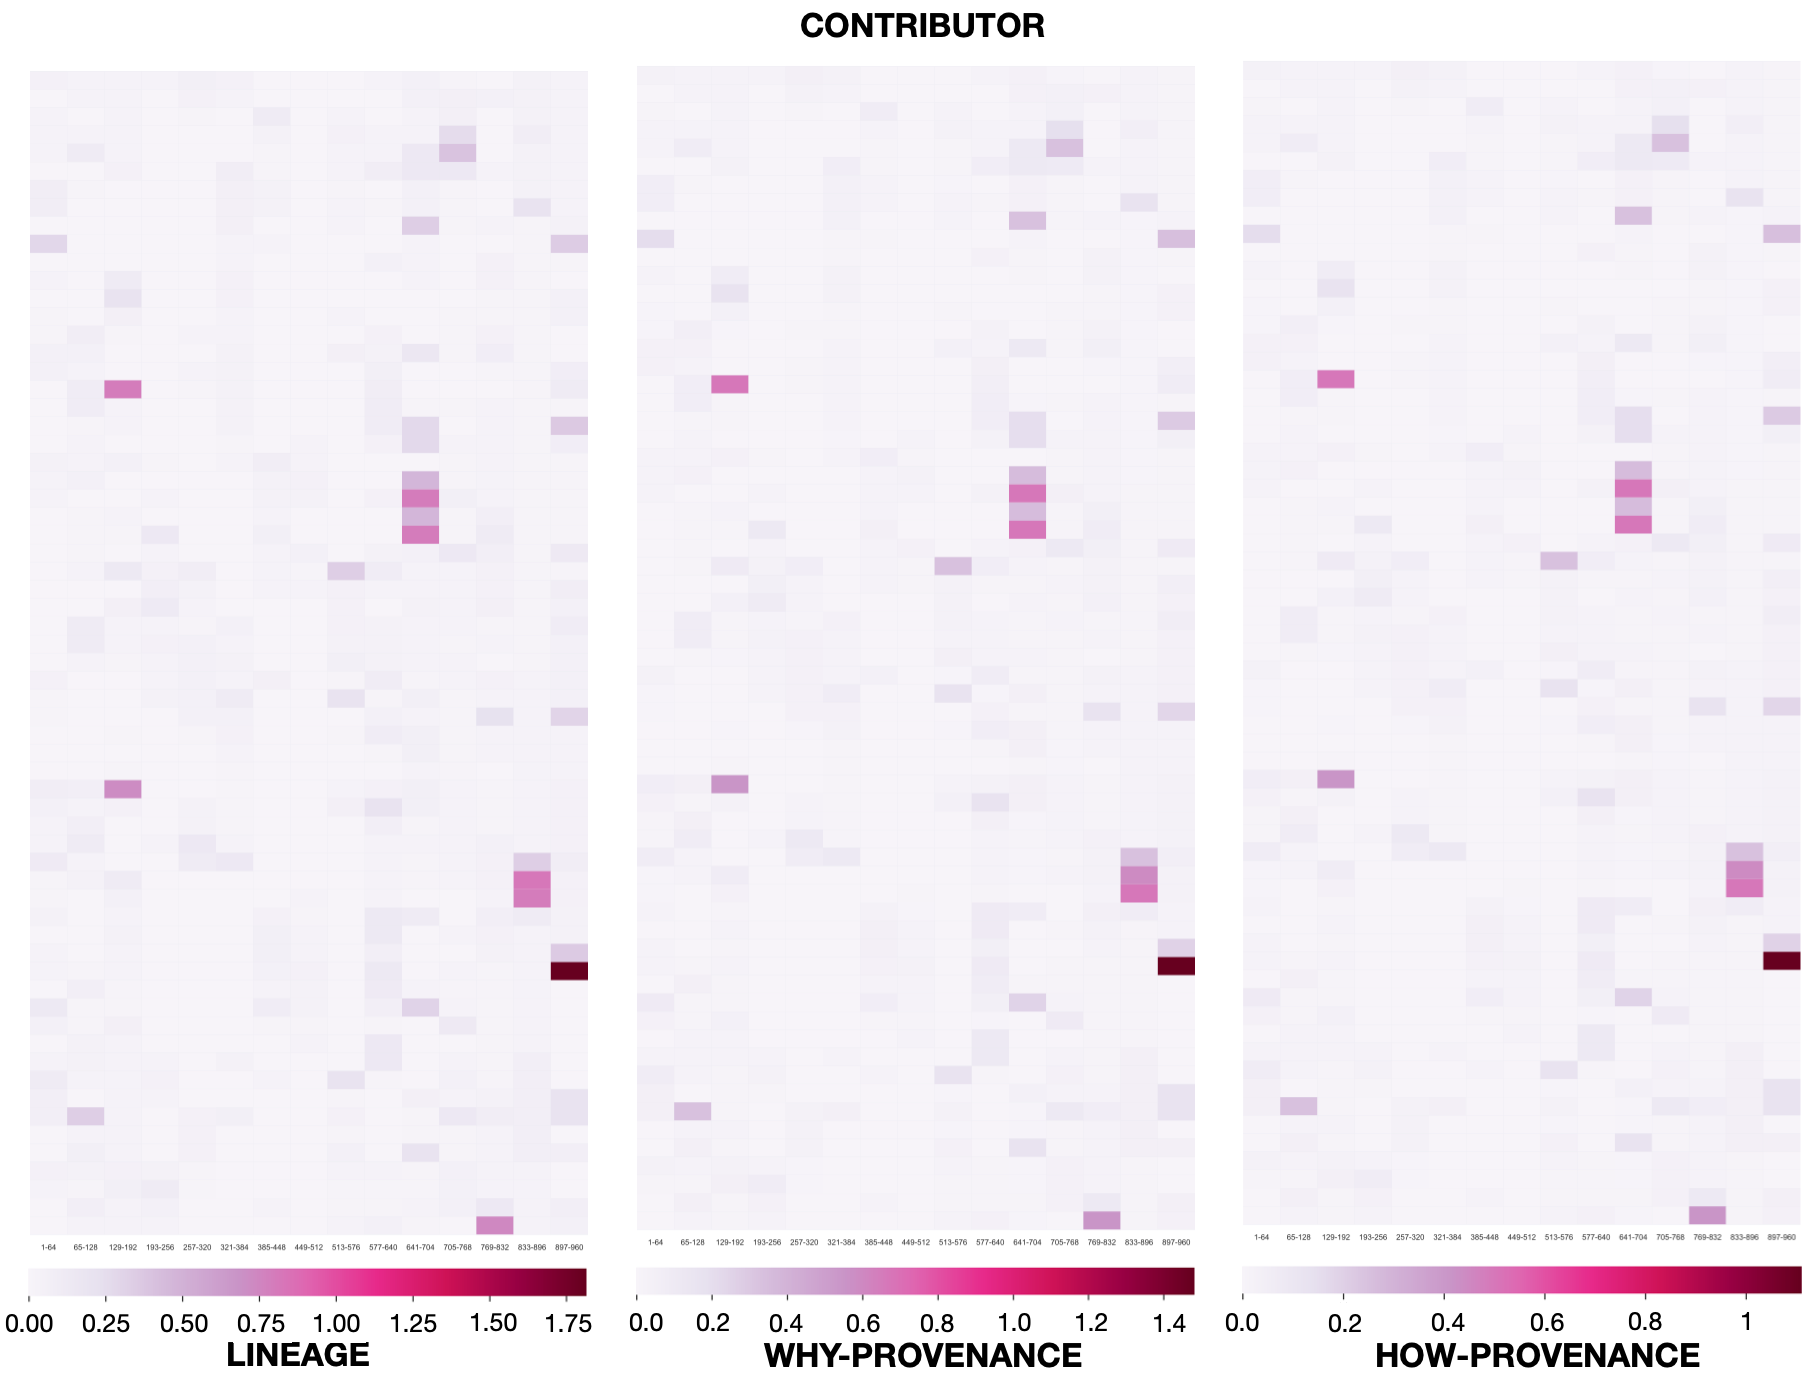
\includegraphics[width=1\textwidth]{figures/synthetic_queries}
  \caption{Comparison of three DS on the same table \texttt{family} after the distribution of the credit connected to query \texttt{Q4}.}
  \label{figure:comparison_on_synthetic_query_1}
\end{figure}

This was only one tuple among the $86$ obtained from this query. If we assign credit $1$ to all these tuples and distribute it with the different strategies, we obtain the result shown in Figure \ref{figure:comparison_on_synthetic_query_1} for the table \texttt{contributor}.
At first sight, it may appear that the three distributions produce the same result. This is only partially true: the heat maps appear equal, but the absolute values assigned to each tuple are different. 
This is more evident if we look at the legend of each heat-map, where the maximum quantity of credit is different for each distribution. The one performed through lineage is around $1.8$, the why-provenance's one is around $1.4$, and the one based on how-provenance is around $1.1$. 

To understand what is happening with this query in this specific table, consider the output tuple \texttt{<Histamine receptors>} and its provenances, as discussed above.
Let us focus on its lineage. There are a total of six authors for this family and $13$ tuples in total in the lineage. 
Thus, using the lineage-based DS, each tuple belonging to the \texttt{contributor} table (i.e. $c_{184}, c_{180}, c_{198}, c_{865}, c_{101}, c_{109}$) receives credit equal to $1/13$.
Tuple $f_{625}$ too receives a portion of credit equal to $1/13$.

Let us consider now why-provenance. Tuple $f_{625}$ appears six times in six different witnesses composed of $3$ elements each. From each witness it receives a portion of credit equal to $1/18$, thus its total credit is $1/3$.
On the other hand, all the authors appear only once in each witness, thus each of them receives credit $1/18$. 
In this case, why-provenance is recognizing more credit to tuple $f_{625}$, since it appears in each witness. The consequence is that this distribution is equally \emph{subtracting} credit from the other tuples in the witnesses and giving it to $f_{625}$. 
In Figure \ref{figure:comparison_on_synthetic_query_1} we are only looking at table \texttt{contributor}. 
This same effect is reproduced for each tuple of the output of query \texttt{Q4}, thus the \emph{absolute} credit values on the tuples vary depending on the deployed strategy. 
What happens is that the tuples in table \texttt{contributor} receive less credit than the one received using lineage, but in the same proportions. The heat map appears thus equal to the one obtained with lineage.
This same effect is also present with the how-provenance-based CDS. In this case, tuple $f_{625}$ is rewarded even more, since it appears with an exponent 2 in each monomial, thus attracting even more credit. 

This is also why when we look at the legend for each part of Figure \ref{figure:comparison_on_synthetic_query_1}, the maximum value reached with the lineage-based DS is higher than the one reached with the why-provenance-based DS, which in turn is higher than the one obtained with the how-provenance. This is because the different strategies reward less and less the tuples of table \texttt{contributor} and more the ones in table \texttt{family}. 

This clearly shows the ability of the different strategies to adapt to situations. All three of them can highlight the relevant tuples in the table. However, they differ in the way they reward the tuples. 
Depending on the task, one provenance can be preferred to the other. 
If the only interest is to highlight the relevant tuples, lineage is sufficient. 
If the interest is also to reward more the tuples that are fundamental to the output, one can also choose why- or how-provenance, knowing that how-provenance rewards even more than why-provenance the relevant tuples that are indispensable for the output.  

\end{comment}


\subsection{Synthetic queries}
\eat{
let us consider the case reported in Figure \ref{figure:comparison_on_synthetic_polynomials_2}. 
The figure reports a distribution of credit performed on the table \texttt{family} through the generation of 10K \emph{synthetic} polynomials. 
We randomly generated provenance polynomials that might be the how-provenance of randomly generated synthetic queries, using the three GtoPdb tables \texttt{family}, \texttt{contributor2family}, and \texttt{contributor}. 
An example of a synthetic polynomial that will be used throughout this subsection is:
}

To simulate synthetic queries, 
%highlight the differences between the three DS, 
we randomly generated provenance polynomials in which the coefficients and exponents could be greater than $1$
%that might be the how-provenance of randomly generated synthetic queries, 
over three GtoPdb tables: \texttt{family}, \texttt{contributor2family}, and \texttt{contributor}. An example can be found in Figure~\ref{fig:syntheticDistributions}, which shows a sample synthetic provenance polynomial (the how-provenance) and the corresponding why-provenance and lineage expressions.  The resulting credit distribution for each DS is shown after the provenance expression. 



\begin{figure}
{\footnotesize{\bf How-provenance:}
$
3 f_1^3 c2f_1^2 c_1^2 + 2 f_1 c2f_2^3 c_2^3 + 4 f_5 c2f_{17}^4 c_{18}^3
$ }\\
\hspace{0.5in} 
{\footnotesize{\bf Credit distribution:}\\ $f_1 = \frac{59}{315}, f_5 = \frac{1}{18}, c2f_1 = \frac{2}{21}, c2f_2 = \frac{2}{15}, 
c2f_{17}=\frac{2}{9} , c_1 = \frac{2}{21}, c_2 = \frac{2}{15}, c_{17} = \frac{1}{6} 
$
}
\\
\\
{\footnotesize{\bf Why-provenance:}
$
\{ \{f_1, c2f_1, c_1\}, \{f_1, c2f_2, cf_2\}, \{ f_5, c2f_{17}, c_{18}\} \}
$ 
}
\\
{\footnotesize{\bf Credit distribution:}\\
$
f_1 = \frac{59}{315}, f_5 = \frac{1}{18}, c2f_1 = \frac{2}{21}, c2f_2 = \frac{2}{15}, 
c2f_{17}=\frac{2}{9} , c_1 = \frac{2}{21}, c_2 = \frac{2}{15}, c_{17} = \frac{1}{6} 
$
}
\\
\\
{\footnotesize{\bf Lineage: }
$
\{f_1, f_5, c2f_1, c_1, c2f_1, c2f_2, c2f_{17}, c_1, c_2, c_{18} \}
$}
\\
{\footnotesize{\bf Credit distribution:}\\
$
f_1 = \frac{1}{8}, f_5 = \frac{1}{8}, c2f_1 = \frac{1}{8}, c2f_2 = \frac{1}{8}, 
c2f_{17}=\frac{1}{8} , c_1 = \frac{1}{8}, c_2 = \frac{1}{8}, c_{17} = \frac{1}{8} 
$}
 \caption{Sample synthetic provenance polynomial (how-provenance) and corresponding why-provenance and lineage expressions with credit distributions}
 \label{fig:syntheticDistributions}
 \end{figure}

\begin{figure}[tb]
  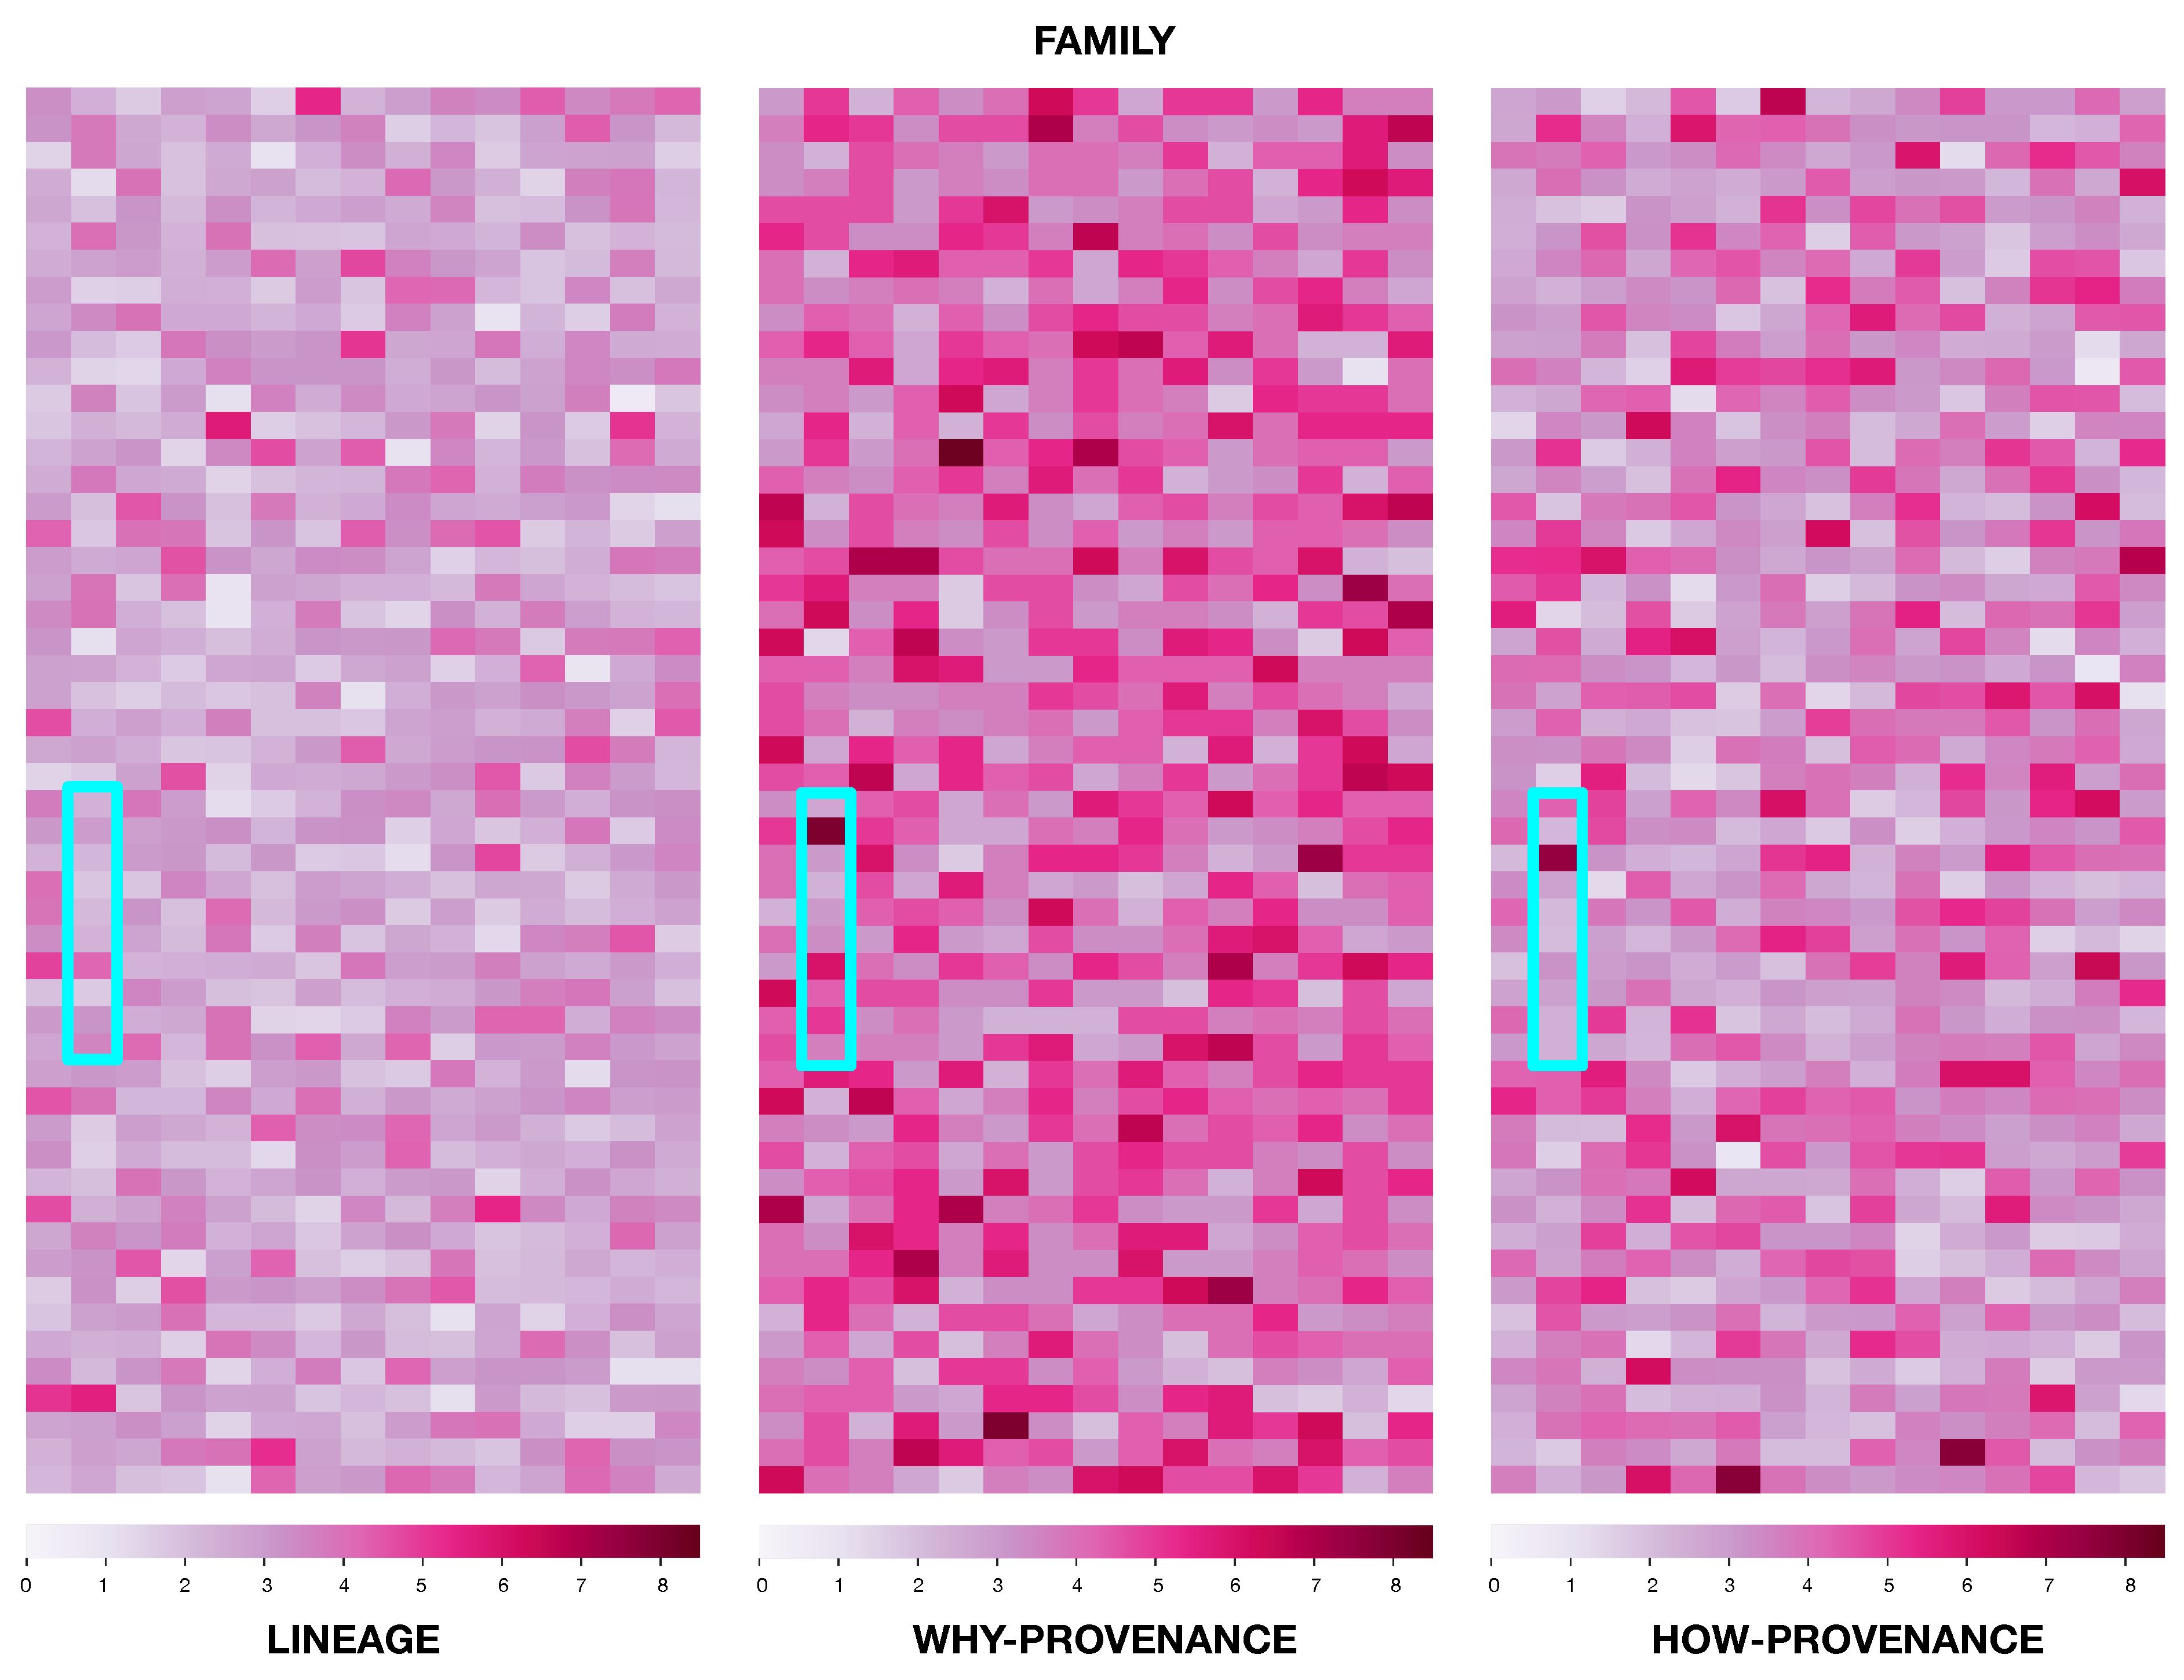
\includegraphics[width=1\textwidth]{figures/synthetic_polynomials}
  \caption{Comparison of three DS on the same table \texttt{family} after the distribution computed using 10K synthetic and randomly generated provenance polynomials. The tuples in the blue rectangles are used as example in the discussion connected to Figure \ref{fig:comparison}.}
  \label{figure:comparison_on_synthetic_polynomials_2}
\end{figure}

\eat{
An example of such a synthetic provenance polynomial is:

{\footnotesize
\[
3 f_1^3 c2f_1^2 c_1^2 + 2 f_1 c2f_2^3 c_2^3 + 4 f_5 c2f_{17}^4 c_{18}^3
\] }
The corresponding why-provenance is: 
{\footnotesize
\[
\{ \{f_1, c2f_1, c_1\}, \{f_1, c2f_2, cf_2\}, \{ f_5, c2f_{17}, c_{18}\} \}
\] 
}
and corresponding lineage is: 

{\footnotesize
\[
\{f_1, f_5, c2f_1, c_1, c2f_1, c2f_2, c2f_{17}, c_1, c_2, c_{18} \}
\]}
 
 Using {\em how-provenance}, the distribution obtained from this sample polynomial is:

{\footnotesize
\[
f_1 = \frac{59}{315}, f_5 = \frac{1}{18}, c2f_1 = \frac{2}{21}, c2f_2 = \frac{2}{15}, 
c2f_{17}=\frac{2}{9} , c_1 = \frac{2}{21}, c_2 = \frac{2}{15}, c_{17} = \frac{1}{6} 
\]
}

Using {\em why-provenance}, the distribution is:

{\footnotesize
\[
f_1 = \frac{2}{9}, f_5 = \frac{1}{9}, c2f_1 = \frac{1}{9}, c2f_2 = \frac{1}{9}, 
c2f_{17}=\frac{1}{9} , c_1 = \frac{1}{9}, c_2 = \frac{1}{9}, c_{17} = \frac{1}{9} 
\]
}


Finally, with {|em lineage}, the distribution is:

{\footnotesize
\[
f_1 = \frac{1}{8}, f_5 = \frac{1}{8}, c2f_1 = \frac{1}{8}, c2f_2 = \frac{1}{8}, 
c2f_{17}=\frac{1}{8} , c_1 = \frac{1}{8}, c_2 = \frac{1}{8}, c_{17} = \frac{1}{8} 
\]
}
}



As an example of how the distribution strategies behave with these synthetic queries, consider tuple $f_5$ in Figure \ref{figure:comparison_on_synthetic_polynomials_2}.
This tuple receives the highest quantity of credit using lineage-based distribution, and less credit using why- and how-provenance because more information is available about the role of the tuple in the overall computation. 
Generally speaking, the more complex the distribution (the most complex being how-provenance), the more credit is given to tuples which are more frequently used or which have a higher impact in producing the output tuple. 

Although synthetic, these provenance polynomials represent realistic queries.  The polynomials can be obtained by any nested query with join and union operations that use the same tuple multiple times (in which case the exponents are bigger than $1$), and the same combination of operations more than once (in which case the coefficients of monomials are bigger than $1$). 

\paragraph{Results} The results of credit distribution on the \texttt{family} table using 10K randomly generated synthetic provenance polynomials are shown in
Figure \ref{figure:comparison_on_synthetic_polynomials_2}. 
We set the maximum value in the heat maps to the highest value reached by a tuple in all three distributions (i.e., $8.33$). 
As can be seen, the three strategies generate significantly different credit distributions indicated by the varying hues.  

Lineage-based DS gives the least credit to tuples in the \texttt{family} table, indicated by an overall lighter hue. This is because the DS equally distributes credit to all tuples appearing in the lineage. Since these queries also use two other tables, credit is distributed to tuples in those tables.

Moving to %the heat-map reporting the distribution performed by the DS based on 
why-provenance-based DS, we see that more credit is given to tuples in the \texttt{family} table than either of the other two strategies, indicated by the overall darker hue. This is because the DS considers the different ways that a tuple is used, e.g. in joins with other tuples. If the same tuple is present in more than one witness, it will draw more credit and take it from  other tuples in the witness basis. In this case, tuples in \texttt{family} drew more credit, taking it from tuples in the other two tables, due to the role that \texttt{family}  tuples played in the queries that were executed.

\scream{Dennis, rewrote, please check for accuracy.}
Finally, consider the how-provenance-based DS heat-map. %  in Figure \ref{fig:comparison}. 
As with why-provenance, more credit is typically given to tuples in \texttt{family} compared to lineage-based DS since it recognizes the role of these tuples in the queries, and the overall hue is deeper.  However, the distribution does not reward all tuples in the same way, since it uses all information contained in the provenance polynomials.  Referring to the ten tuples within each large blue rectangle (each small rectangle within the large blue rectangle is a tuple), we will number them from 1 (top) to ten (bottom).  Note that tuples 2, 7, 8, and 9 are awarded less credit than in either the lineage- or why-provenance strategies, whereas tuples 1 and 3 receives more credit than either of the other two strategies. 
\eat{
However, the distribution does not reward tuple 2 in the same way. Also tuples 7, 8, and 9 that appear to be rewarded heavily in the why-provenance-based DS here are contain lower quantities of credit. Vice-versa, tuple 3 is much higher in credit with respect to what happens with the why-provenance-based DS.
This is due to the fact that this DS is even more sophisticated, since it uses all the information contained in the provenance polynomials. 
In this case, a tuple as 3 is able to attract even more credit than before. However, other tuples, such as 2, 7, 8, and 9 receive now less credit, since they role appears to be less determinant once the full information from the polynomials is taken into considerations. }
This shows in more detail that the DS based on how-provenance is more nuanced in terms of credit distribution than the other strategies. 
\eat{even more sophisticated, and can be taken into consideration when a user wants to distribute credit with a higher level of sensibility.}
%\textbf{ $\leftarrow$  Gianmaria: This is not clear and I suggest a rewriting of this paragraph.}

%%%%%%%%%%%%%%%%%%

\subsection{Credit accrual over time} 
Since credit accrues over time, we simulate the passage of time by varying the number of queries executed, and look at the ``snapshots" of credit for each of the strategies using synthetic queries.  The results are shown in Figure \ref{fig:comparison}.

\begin{figure}[t]
  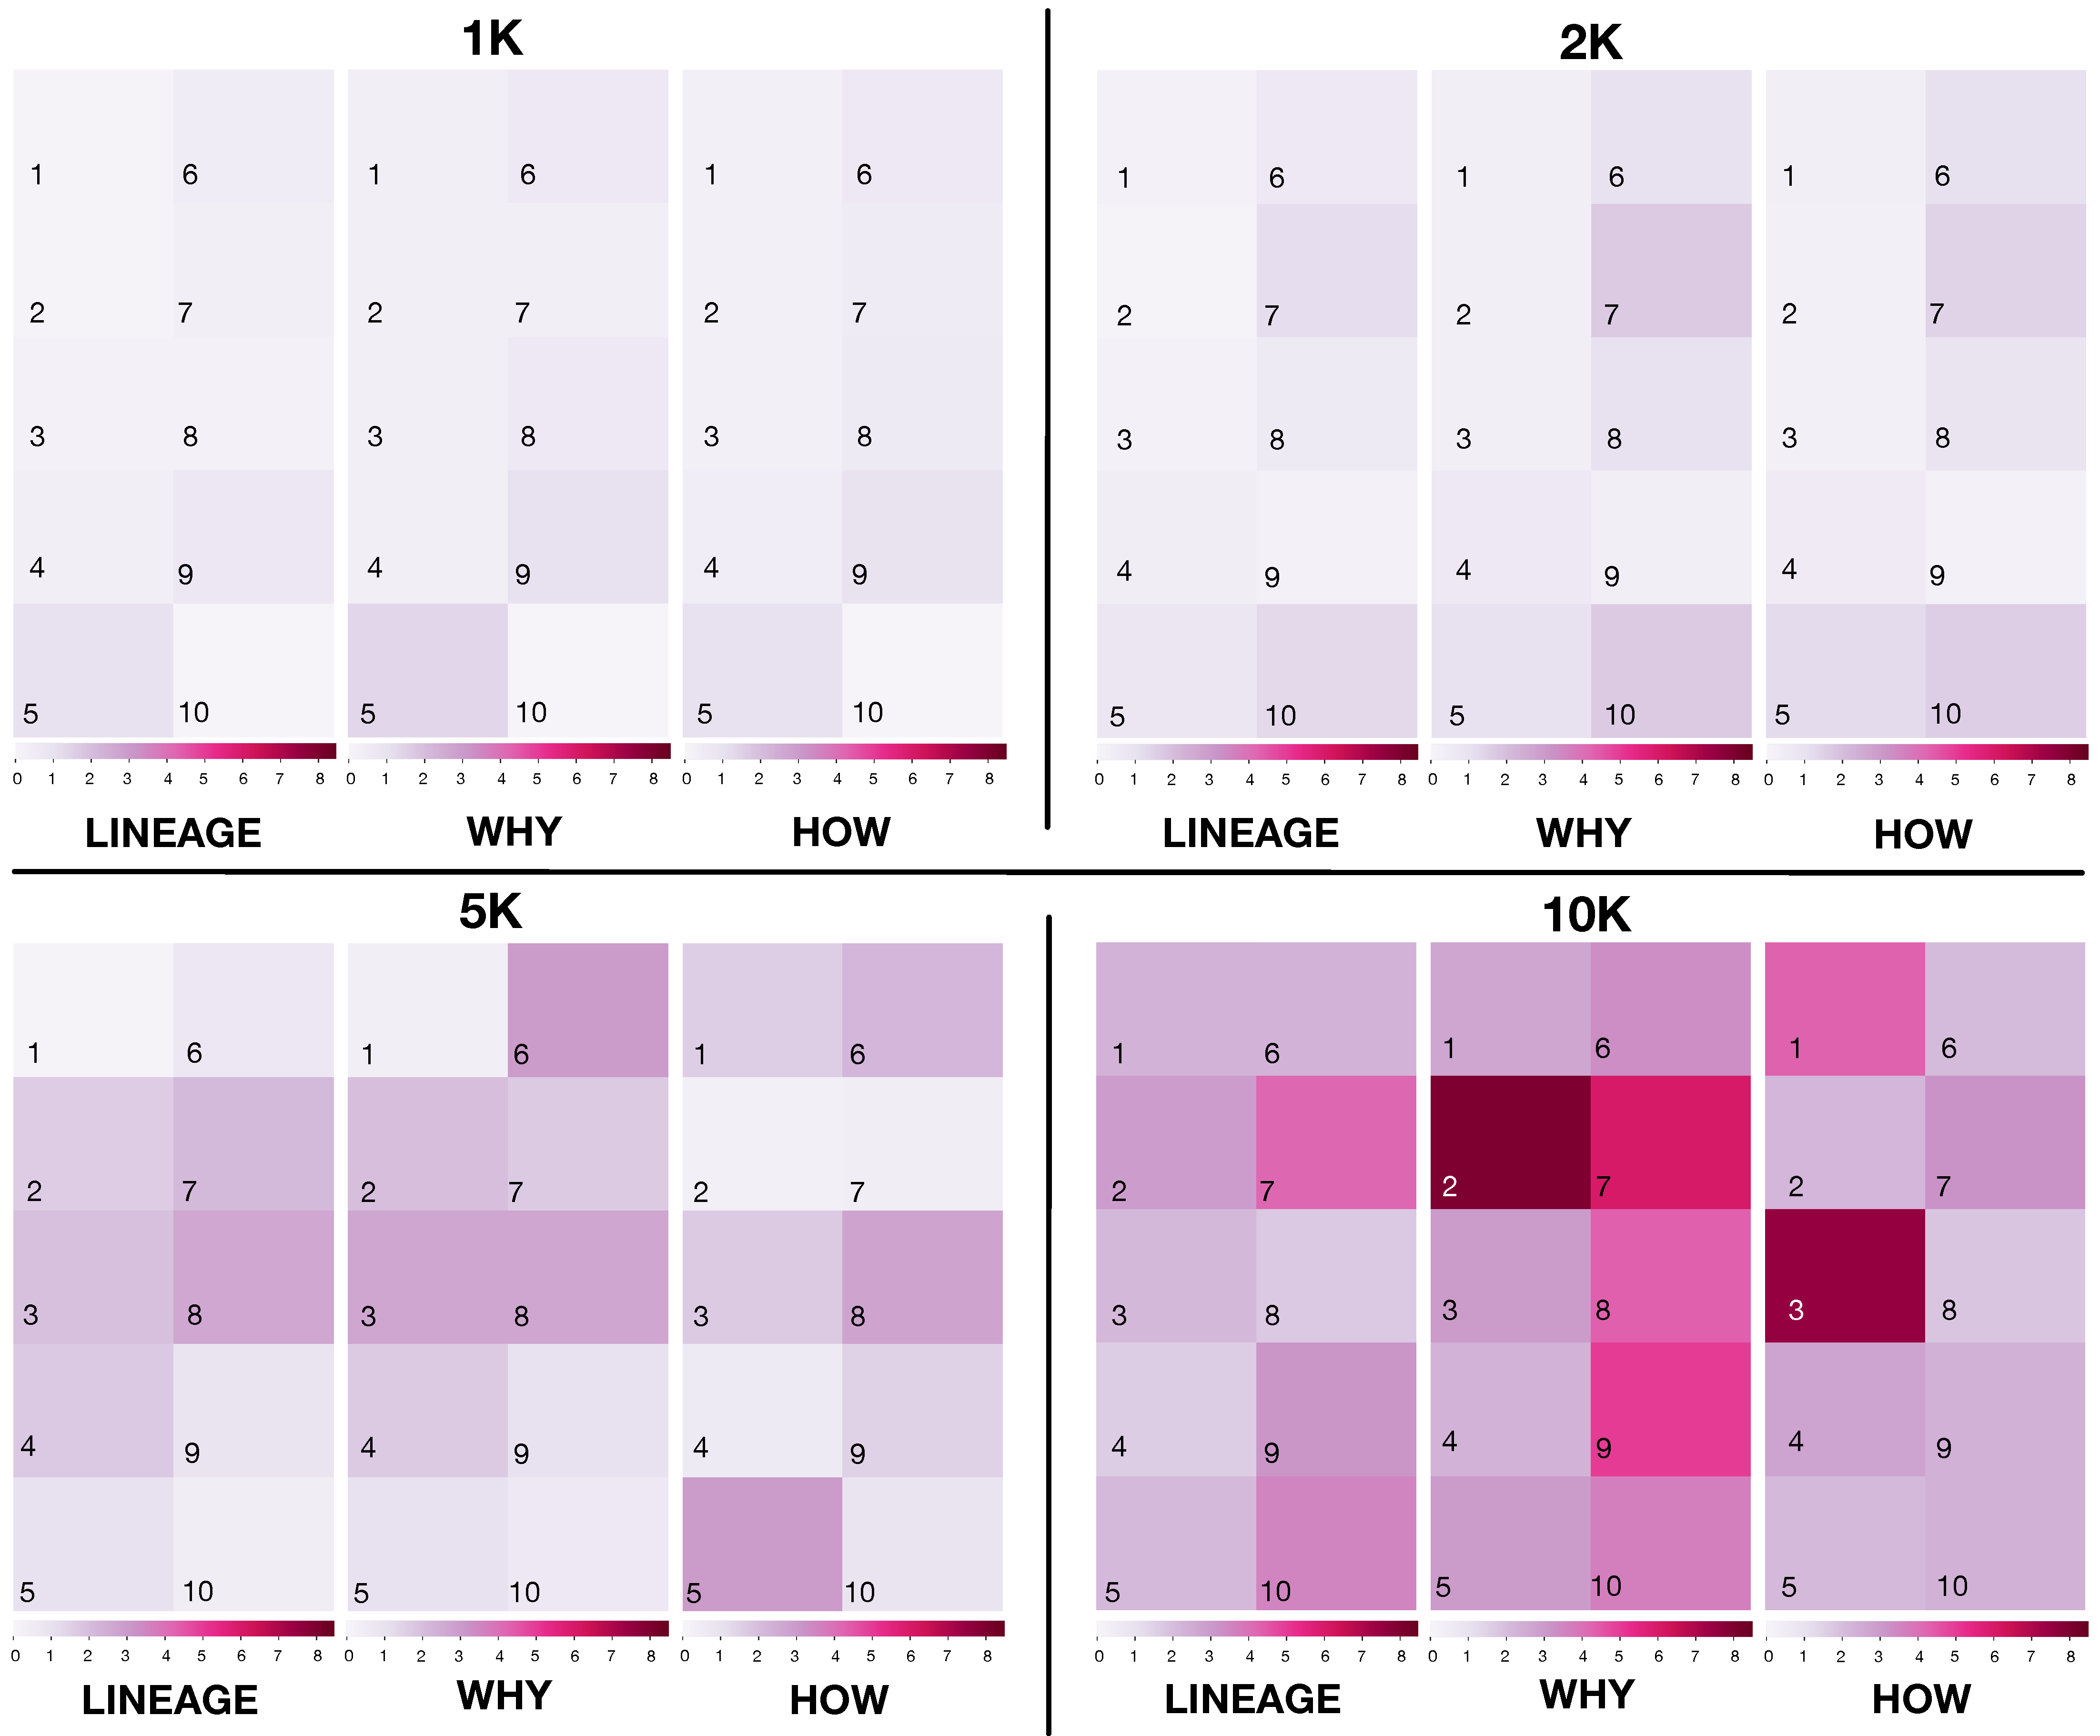
\includegraphics[width=\textwidth]{figures/comparison_2}
  \caption{Comparison of the distribution of credit performed by the three DSs on a subset of 10 tuples taken from the \texttt{family} table, simulating the passing of time. The number at the top of each group of heat-maps represents the number of queries.}
  \label{fig:comparison}
\end{figure}

\scream{Dennis:  What is the "rank" of tuple about, and why do we need to bring it up? I've taken it out, see if this is still correct.}

In this figure, four groups of heat-maps are shown. Each group represents a ``snapshot'' taken %during an incremental accumulation of credit on the database 
after 1K, 2K, 5K and 10K queries have been executed.  The ten tuples in each heat-map are from the \texttt{family} table, and are the ones highlighted previously in the blue boxes of Figure \ref{figure:comparison_on_synthetic_polynomials_2}.  
\eat{The heat-maps maps are over the ten tuples from the GtoPdb \texttt{family} table after an incremental distribution of credit (the tuples of ranks ranging from 79 to 89). These are the same tuples highlighted in the blue boxes in Figure \ref{figure:comparison_on_synthetic_polynomials_2}. 
Figure \ref{figure:comparison_on_synthetic_polynomials_2} represents the end of the process.  }
\eat{
In this way, we simulate the passing of time on a database where credit distribution is performed. Each group of heat-maps can be thought of as a snapshot of that set of tuples at a certain moment. }
The queries used are the same as the experiment reported in the previous section. The range of credit in each map goes from 0 (no credit) to 6 (the maximum quantity of credit reached on a tuple at the ``snapshot'' with 10K queries).


Focusing on the 1K and 2K groups, we see that credit distribution by the three DS are very similar. Still, there are small differences, in particular in tuple 5.
\scream{Dennis: need to say more about tuple 5. Why not also 7 and 10? The interesting one to me is tuple 9, whose credit appears to decrease.}


The first interesting differences come after 5K queries. In particular, note how tuple 7 receives very little credit in the lineage-based DS, more in the why-provenance-based DS, and the most credit in the how-provenance-based DS. This is because tuple 7 appears in a relatively few lineages, but its role is critical to these queries; thus, why- and how-provenance-based strategies reward it more.
On the other hand, tuple 5 is highly rewarded by the lineage-based and why-provenance-based DSs, and less by how-provenance. Although tuple 5 appears in many queries and is used in different combinations, its exponents in the provenance polynomials is low, therefore giving it less credit with how-provenance than with why-provenance.
\scream{Dennis:  What does "tuple 7 appears in a relatively few lineages" mean?  Do you mean it appears in relatively few results, but plays a crucial role?}

\scream{Dennis: I don't understand this paragraph at all.  I am stopping here in this subsection until you clean this up a bit, it's very confusing. }
It is also interesting to note how other tuples like tuple 2 now surpass certain tuples, like tuple 1 that up to 2K queries presented the highest values of credit. This shows how credit can keep track of the ``hotspots'' in a database over time. The presence of new queries and new credit distributions can change the hotspots in a table, showing how the research community's interests may change during time. 

Finally, the largest differences are shown in the 10K group. In this case, we see a situation similar to the one with 5K queries. Like 8 or 10, specific tuples receive more credit with why-provenance and how-provenance, rather than with lineage. This is still due to the critical role of the tuple in the queries where it appears. 

From this progression, given the particular synthetic provenance polynomials that were presented, we can see the differences between the three distributions. These differences become more evident with time, i.e., the more credit is distributed to the tuples. 

%Therefore, although all the three considered DS considered here are effective in distributing credit, they actually behave differently. 
The DS based on lineage is sufficient when a user only wants to highlight the tuples of the database used by a query (and not only visualized in the output). However, it equally distributes the credit to the tuples of the lineage, therefore not considering the information on the tuples' role in the production of the output. 

For this reason, a user may want (depending on the nature of the queries) to use DS based on why-provenance and how-provenance. %These two DS are sensitive than the DS based on lineage (and the DS based on how-provenance is more sensible than the one based on why-provenance). 
Using the why-provenance and how-provenance DS, it is possible to change the distribution of credit to the tuple, rewarding more the tuples that have a more critical role in generating the output. Therefore, these two DS can be preferred when the user aims to find ``hotspots'' in the database based on the tuples' role. 

%In particular, the DS based on why-provenance rewards more the tuples that are used in different ways by queries (i.e. are members of more witnesses). The DS based on how-provenance also takes into consideration how many times a tuple is used, adding even more sensibility to the distribution. 
%One may choose one other the other depending what are the aspects he wants to highlight in the data.

%%%%%%%%

\subsection{Credit vs Citations}

\begin{figure}[]
\centering
  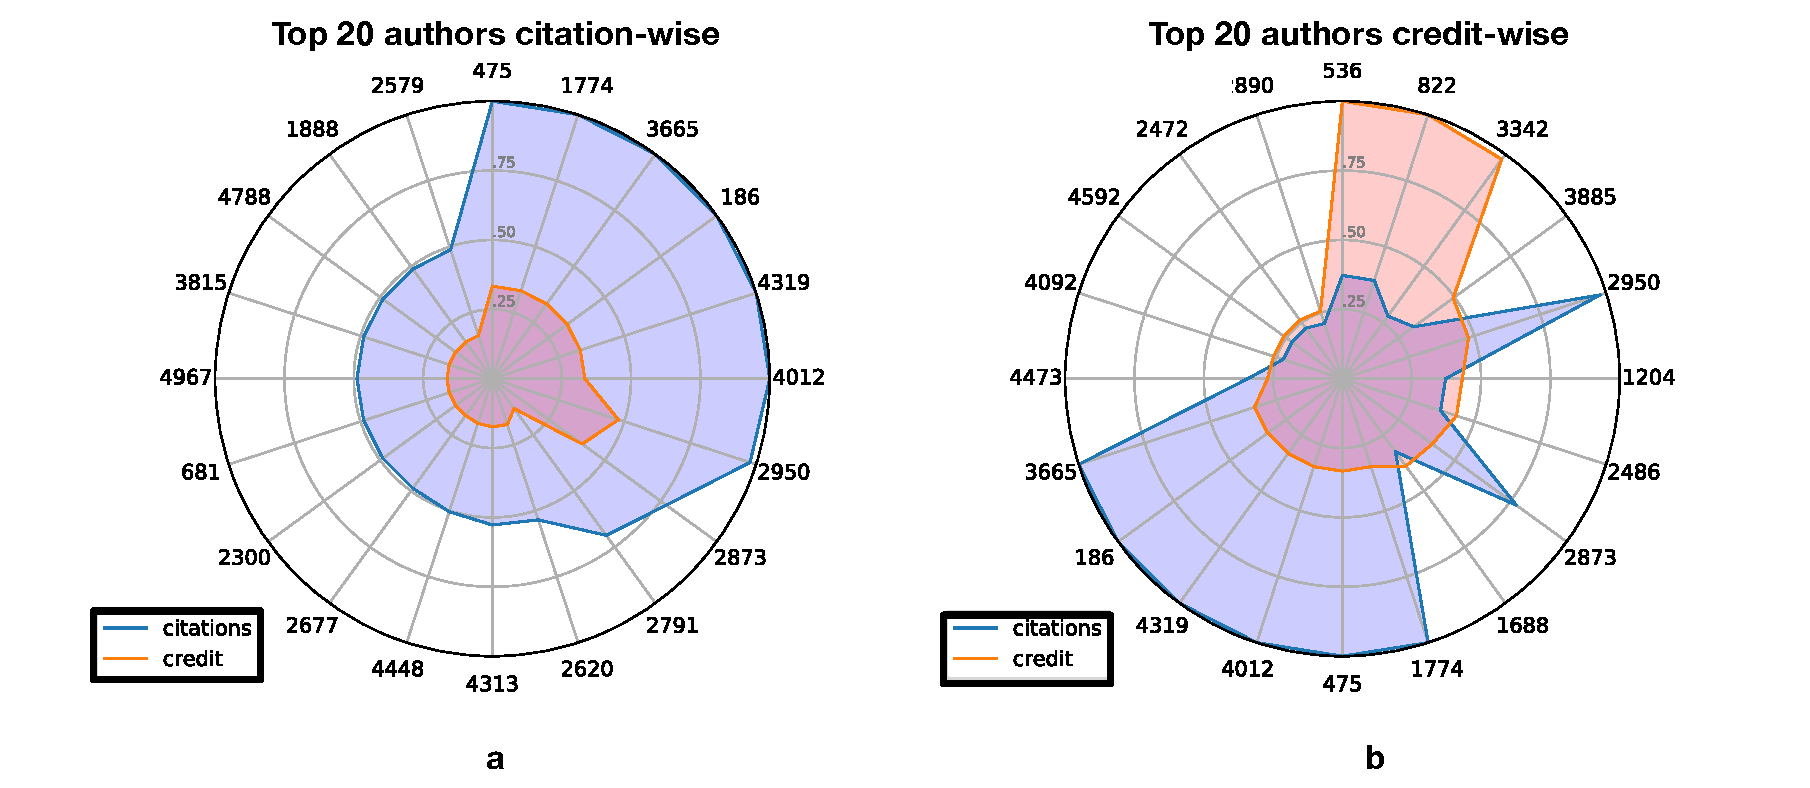
\includegraphics[width=1\textwidth]{figures/2_radars}
  \caption{Radars presenting the top 20 authors citation-wise and credit wise, together with their (normalized between 0 and 1) values of citations and credit.}
  \label{figure:2_radars}
\end{figure}

\scream{What is the set of authors, just ones on papers in BPC or are they the data curators?  Check if what I say below is correct!}

In the last set of experiments, we compare credit generated by traditional citations and the proposed credit distribution strategies to see the difference in reward for authors, including data curators.  
The set of authors used in the experiments are \scream{??} those appearing on the paper traditionally cited for GtoPdb, as well as data creators and curators in the \texttt{contributor} table in GtoPdb responsible for producing the data used in the queries.  An author receives credit via a traditional citation when the traditional GtoPdb paper is cited; they receive credit via a DS when data which they created or curated receives credit.
We perform the comparison using both real-world and synthetic queries.

\paragraph{Results: Real-world queries}
As described in Section \ref{sec:real_world_queries}, the real-world queries are taken from papers published in the BJCP which reference webpages in GtoPdb.
Since for these queries there is no difference in the distribution of credit between the three DS, only one value for credit is given.

The results are shown in the radar plots of Figure \ref{figure:2_radars}, in which each number on the outer circle (e.g. 475, 1774 and 3665) represents an author (id) and the blue (pink) line represents the normalized value of credit generated by citations (credit), respectively. The first radar plot,
Figure \ref{figure:2_radars}.a, orders the top 20 authors based on citations in a clockwise direction, whereas Figure \ref{figure:2_radars}.b, orders the authors with the highest value of credit who do not also have the highest number of citations. \scream{what does that mean?  and it seems that there is not a large overlap in the authors in fig. a and b}

\eat{The results are shown in the radar plots of Figure \ref{figure:2_radars}.
Figure \ref{figure:2_radars}.a reports the top 20 author (we identify the authors with their ID instead of their name), ordered based on the normalized value of citations distributed by the queries taken from the papers published in BJP as described in Section \ref{sec:real_world_queries}, together with their normalized value of credit. 
An author transitively receives credit from the data s/he created or curated. The credit assigned to data is then split equally to the authors of those tuples. 
As shown in Section \ref{sec:real_world_queries}, there is no difference for these queries in the distribution of credit between the three DS. Thus these values are equal for the three distributions.  }

The second radar plot, Figure \ref{figure:2_radars}.b, orders authors based on the quantity of credit. 
\scream{Shoudl discuss that this is not necessarily the same set of authors?}
As can be seen, the quantity of credit and the number of citations differ significantly:  An author with a high number of citations may have a low credit value (e.g. 475). Similarly, an author with a high credit value may have a low number of citations.  \scream{I didn't see any to point to in the figure... and I didn't understand the next few sentences, please reword.} 
This means that there are citations that are more ``valuable'' for an author regarding credit. This is because the quantity of credit assigned by these citations is very high, i.e., the impact of those cited data is high. Authors that are cited less than others can have, nonetheless, a high impact on the research community and thus receive a higher quantity of credit.



%\begin{figure}[t]
%\centering
%  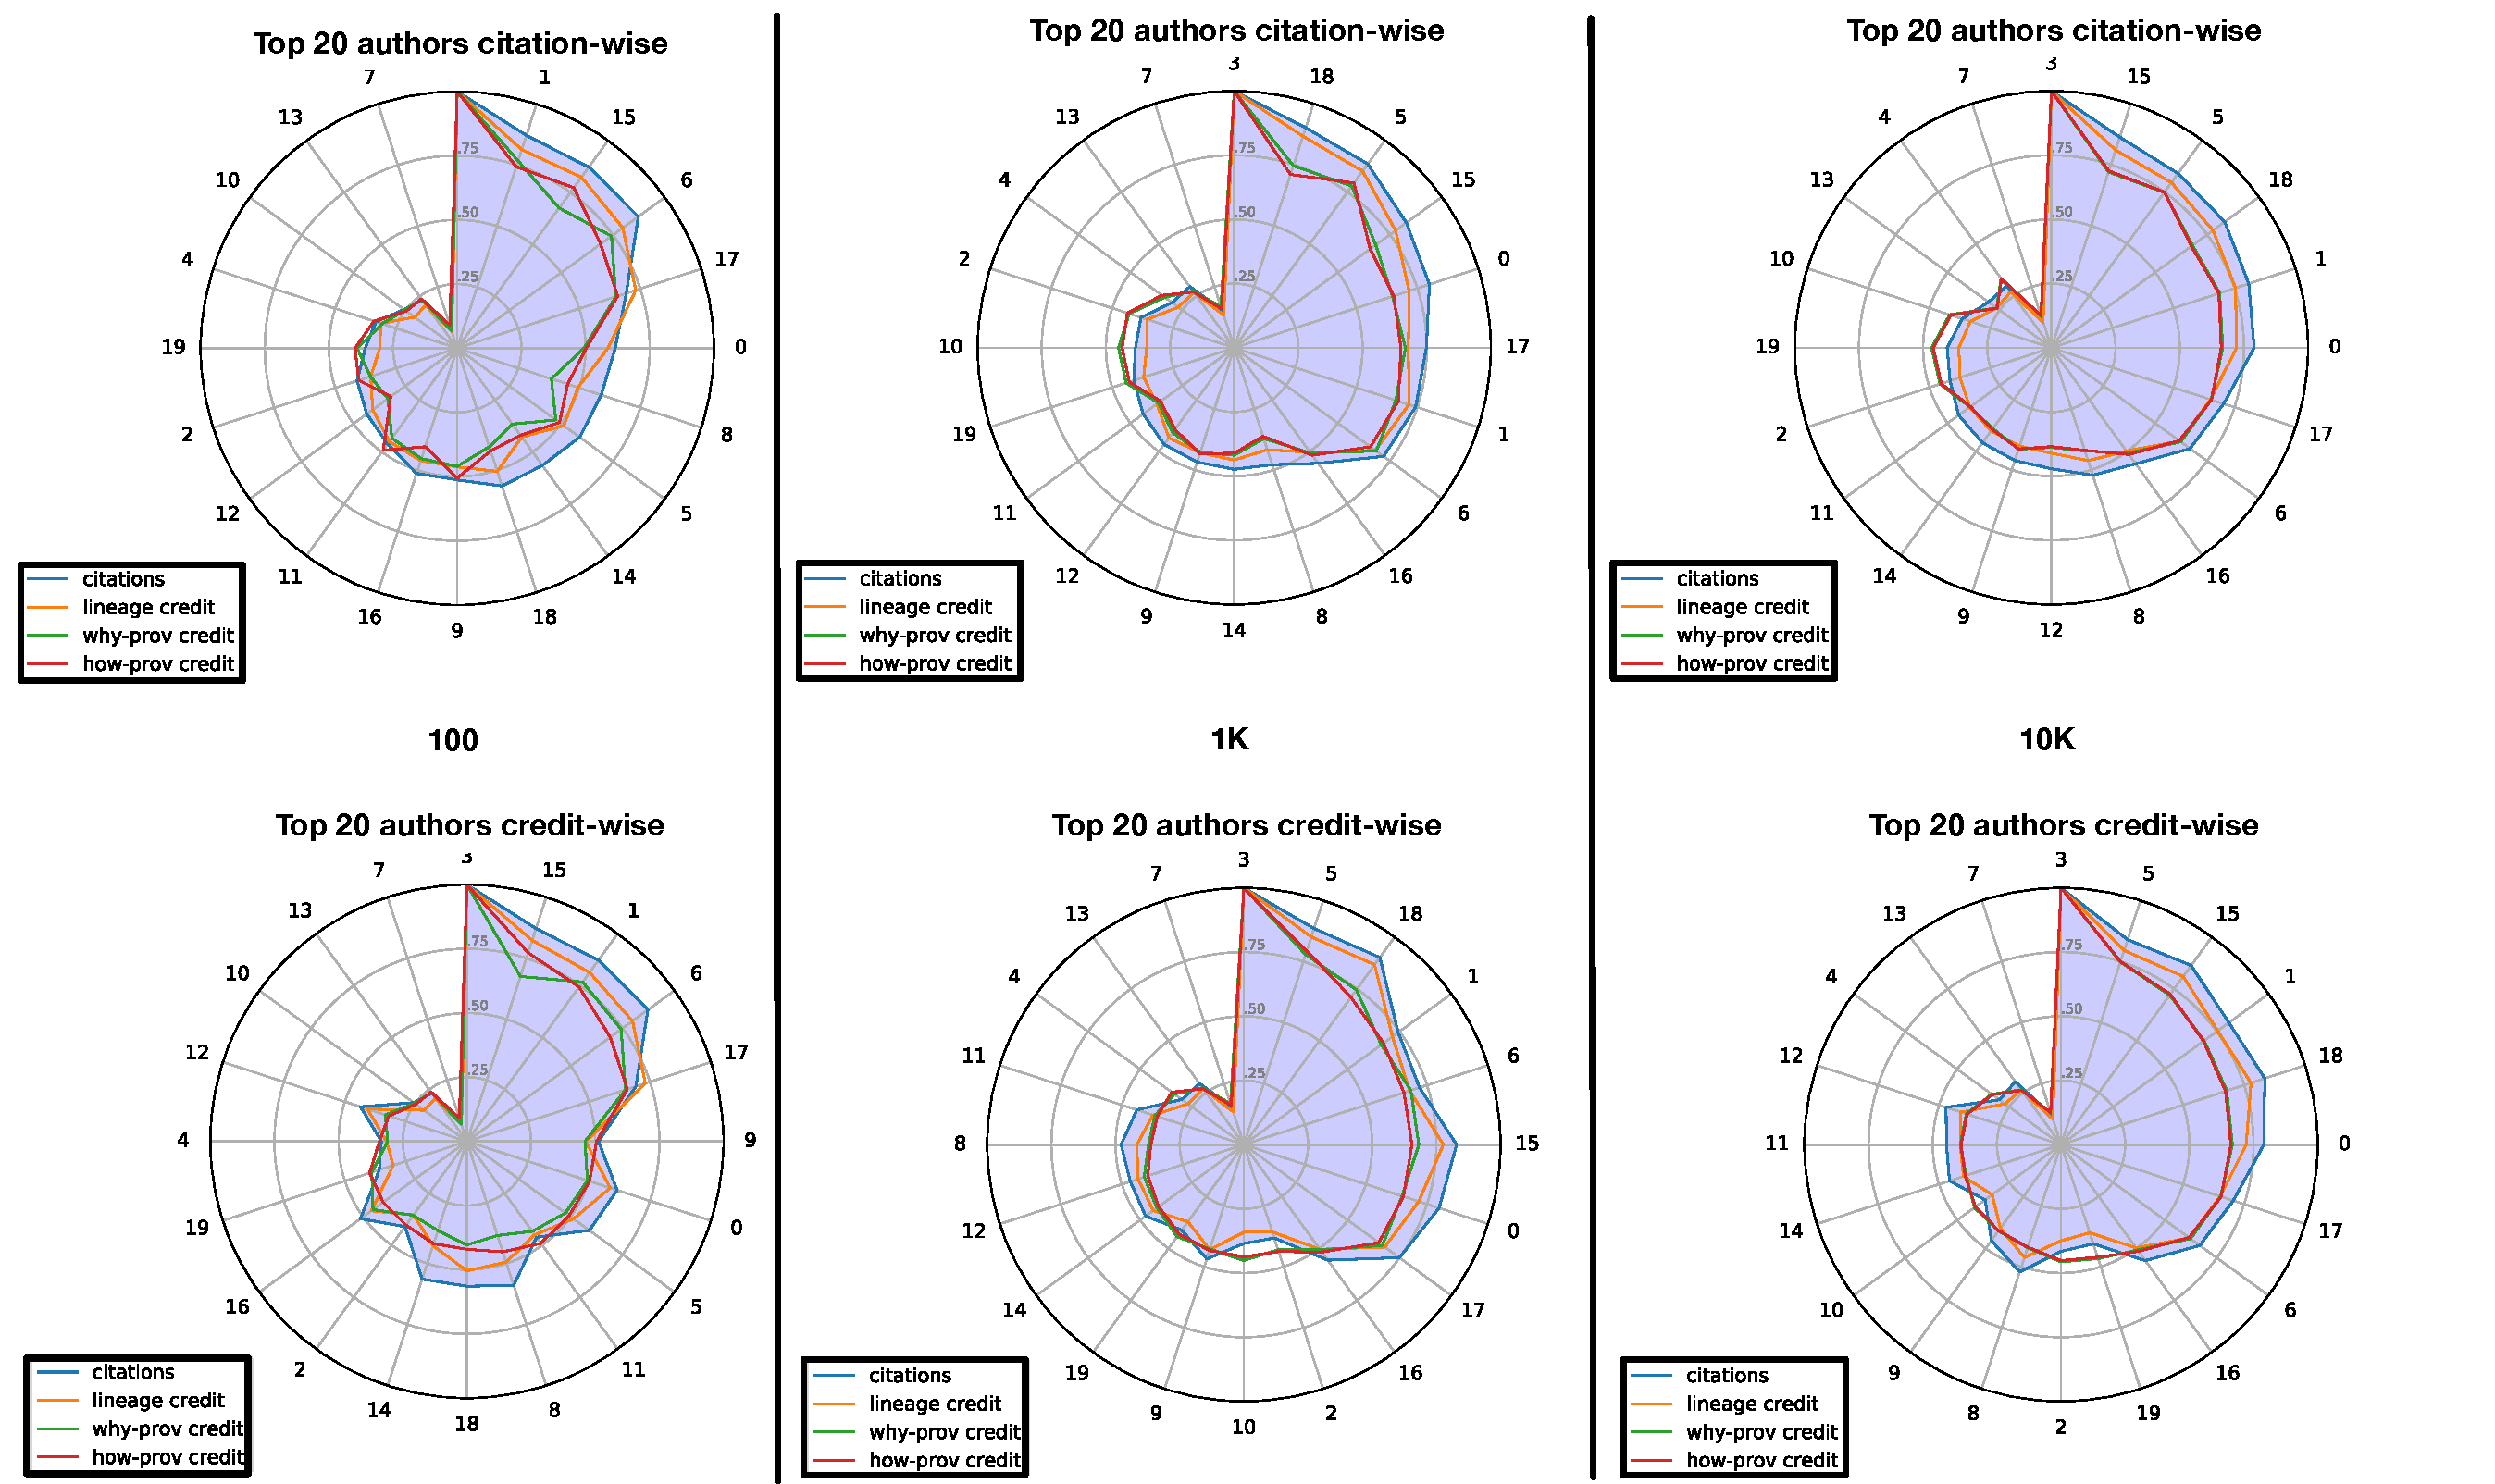
\includegraphics[width=1\textwidth]{figures/3_radars}
%  \caption{Radars presenting 20 authors ordered citation-wise and credit-wise, together with their (normalized between 0 and 1) values of citations and credit, through the execution of different numbers of polynomials (100, 1K, and 10K). The radar plots ordered by credit consider the credit assigned by the DS based on how-provenance.}
%  \label{figure:3_radars}
%\end{figure}

\begin{figure}[t]
\centering
  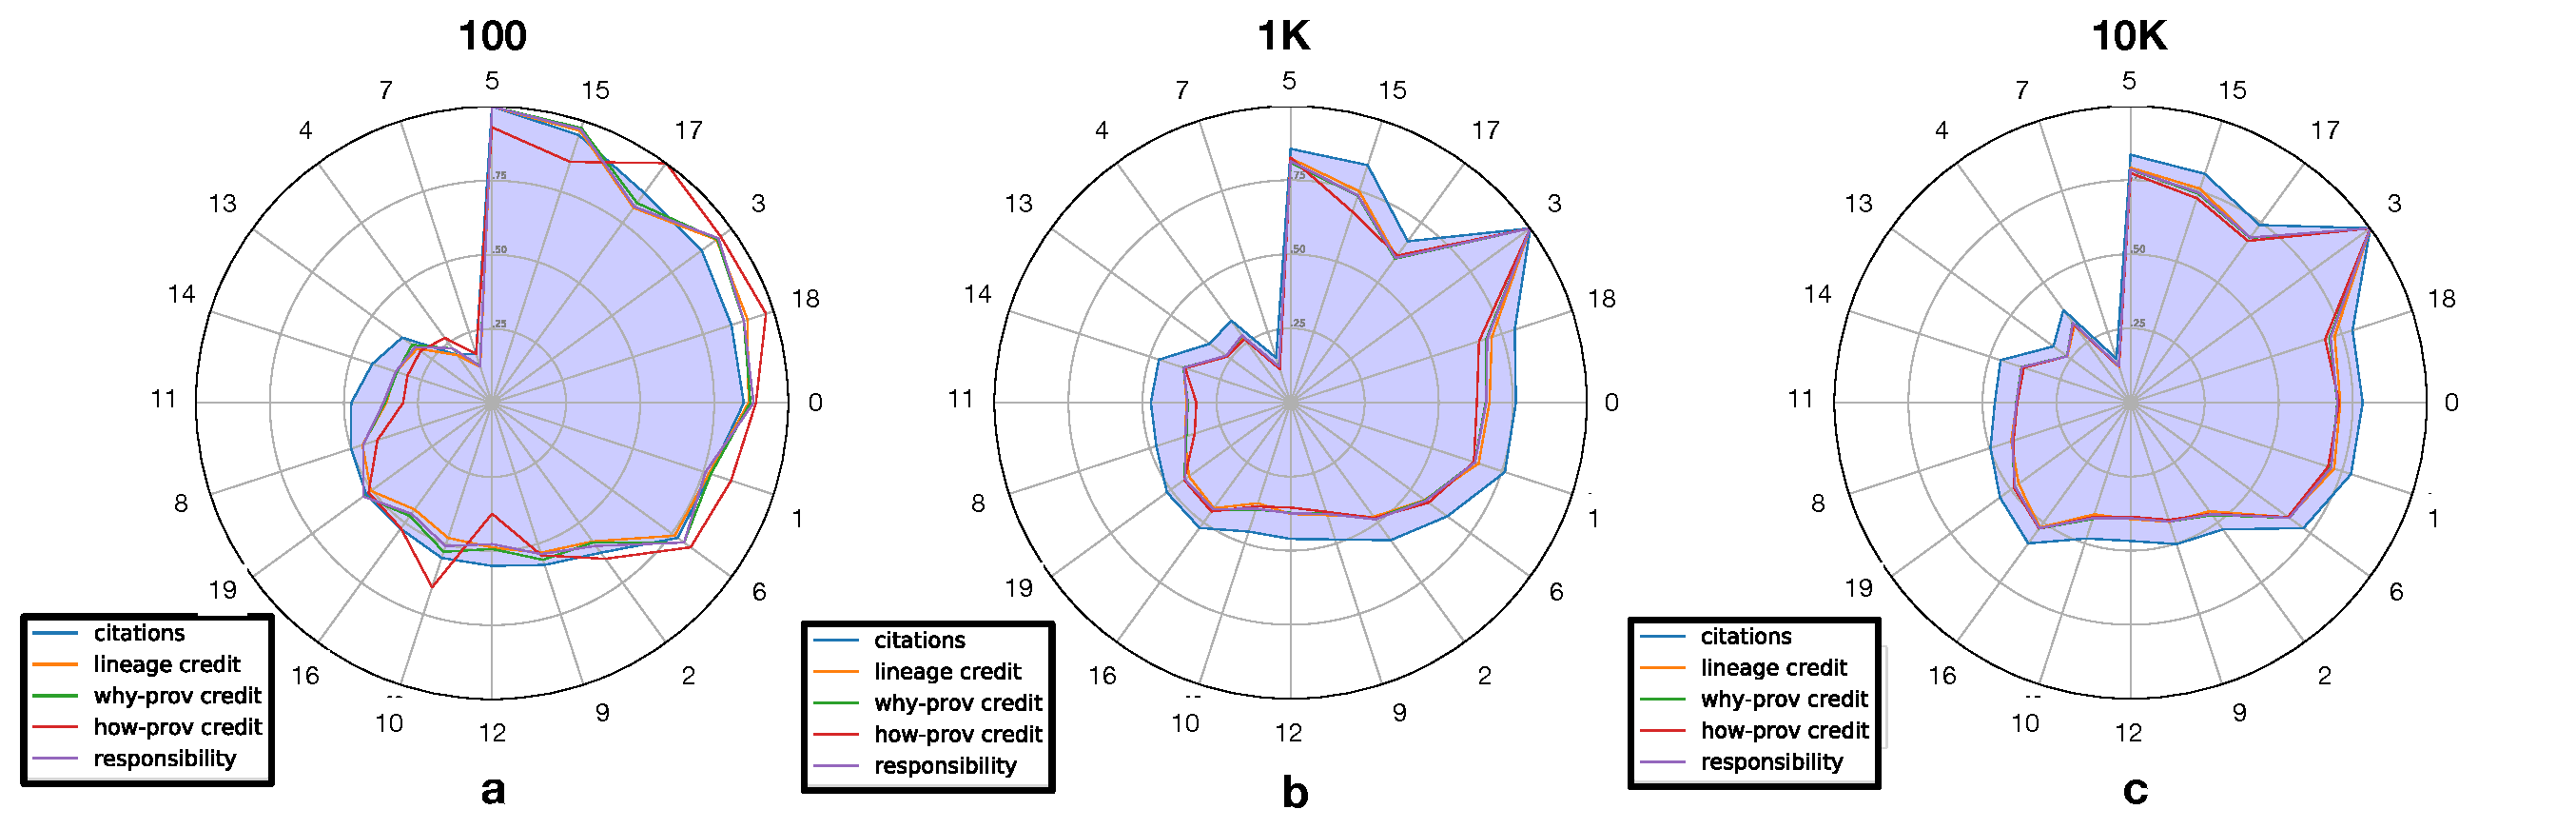
\includegraphics[width=1\textwidth]{figures/fixed_radars}
  \caption{
  Radars presenting the 20 synthetic authors with corresponding citation and quantities of credit distributed through the 3 DS (all values normalized between 0 and 1) through different numbers of polynomials (respectively, 100, 1K and 10K). 
  The order is the descending one of the citations of the authors with 100 polynomials. }
  \label{figure:3_radars}
\end{figure}

\paragraph{Results: Synthetic queries}
We produced $100$, $1K$, and $10K$ synthetic polynomials and distributed credit through them to data. 
\scream{I don't understand the rest of this paragraph.  ARe you saying you can't figure out the creators/curators of the data?  But you were able to do that in earlier experiments, so why not now?  I'm missing something in the setup.}
Since these polynomials correspond to queries whose authors are not easily identifiable, we created $20$ ``synthetic'' authors, and we randomly assigned one author to each tuple in the database. The authors receive ``blocks'' of consecutive tuples, with each block of the size varying between $10$ and $40$ to simulate different quantities of ``work'' performed by an author. 
Every time an author appears as curator of one or more tuples used in a query, we assigned one citation to that author.  
He also receives three kinds of credit, the ones assigned to his tuples through the three different DSs.

Figure \ref{figure:3_radars} reports the three radar plots that are a consequence of the distribution of credit and citations performed and described above with the different quantities of polynomials. 
Figure \ref{figure:3_radars}.a reports the radar plot obtained with 100 polynomials, showing the normalized values of the citation and types of credit assigned to each author. 
As we see, given the synthetic nature of these queries, the correlation between the number of citations and the quantity of credit assigned to the authors appears to be a much stronger with respect to the case with the real-world queries (the linear correlation between the citation number and all three types of credit is always above 0.95 with p values in the order of 1e-11).
Nonetheless, it is still possible to observe how credit does not always exactly follow the citations. 
The credit distributed via lineage is the one that follows closer the number of citations (a linear correlation of 0.98, p value of 6.15e-16), while the other types of credit behave slightly differently (a linear correlation of around 0.95 in both cases).  

Similar observations can be made for Figure \ref{figure:3_radars}.b and \ref{figure:3_radars}.c, where we kept the order of authors as found in Figure \ref{figure:3_radars}.a.

What appears from these figures is that, in certain cases, authors that do not have the highest values of citations receive more credit than others, as for example author 11 in Figure \ref{figure:3_radars}.a, or author 19 in Figures \ref{figure:3_radars}.b and \ref{figure:3_radars}.c, with credit distributed with how-provenance-based DS.

This once again shows how credit allows us to gain a different perspective on the role of data and authors by going beyond the limitations of traditional citations.  

It is worth pointing out that, when scaling up to $1K$ and $10K$ polynomials, the distributions performed via why-provenance and how-provenance become almost equivalent. We can note that, although not exactly overlapping, the values of credit assigned to the authors by those DS become quite similar with these higher quantities of polynomials, suggesting a sort of equivalence between the two DSs in this case, at least in the task of rewarding authors (the linear correlation for the values of Figure \ref{figure:3_radars}.c is more than 0.99 with a p-value of 1.32e-32). 

Since in these experiments we assumed that each output tuple carries credit 1, the queries that return outputs with more tuples also generate more credit.
In Figures \ref{figure:2_radars} and \ref{figure:3_radars} the authors that curated bigger bulks of data also receive higher quantities of credit.
In more complex and sophisticated scenarios, where different strategies may be implemented to decide the generated quantity of credit to be distributed, new factors beyond the only ``quantity'' of curated data can be factored in in rewarding data curators.
The result will be a distribution of credit that represents even better the actual work and worth of data curators.


\subsection{Execution time}

\begin{table}[hbt]
\centering
  \begin{tabular}{| l |c | c | c | c ||}
  \hline
    \# of polynomials  & lineage & why-prov. & how-prov. \\
    \hline
    100 & 226.6 ms & 192.0 ms & 185.5 ms \\
    200 & 431.2 ms & 392.2 ms & 403.2 ms \\
    500 & 1.013 s  & 934.2 ms & 881.8 ms \\ 
    1K  & 2.041 s  & 1.934 s  & 1.744 s  \\
    2K  & 3.773 s  & 3.491 s  & 3.510 s  \\
    5K  & 8.992 s  & 8.653 s  & 8.889 s  \\
    10K & 17.10 s  & 16.84 s  & 16.84 s  \\
    20K & 34.59 s  & 35.30 s  & 39.70 s \\
    100K & 3.289 min & 3.442 min & 3.652 min \\
    1M  & 35.91 min & 34.87 min & 37.91 min \\
    \hline
  \end{tabular}
  \caption{The times required to perform the three DS for different number of synthetic polynomials.}
  \label{table:times}
\end{table}

\scream{Where is this table?  Table 5 does not show times, and I can't find one that does.}
Table \ref{table:difference_result} shows the time required to calculate the credit distribution for the three strategies. As can be seen, the execution time grows linearly with the number of polynomials that are submitted to the system. With a high number of polynomials (1M), the time required by the DS based on lineage and why-provenance is lower than the time needed for the DS based on how-provenance. This is due to the more significant number of operations required to calculate the how-provenance DS  and distribute the portions of credit to be assigned to the different tuples. 
We note that, since we created these polynomials on-the-fly, these values do not include the time required to compute the provenances.
Therefore, limited to the time required to distribute credit, the three DS are equivalent in terms of performances. The first differences can be seen only with high number of polynomials, when lineage and why-provenance may be preferred if there are no requirements to assign credit with the strategy implemented by the how-provenance-based DS.

All the experiments were carried out on a MacBook Pro %13-inch, 2019 
with a 2.4 GHz processor Intel Core i5 quad-core and 8 GB of memory at 2133 MHz.  Code was written in Java, supported by a PostgreSQL database. 


%\subsection{Discussion}
%
%In the previous sections we showed, through the use of different experiments, the behavior of credit and its distribution with the use of different DS. 
%It appeared that, in the case of SPJ queries, the three distributions behave in the same way on GtoPdb. 
%
%Using synthetic polynomials, we showed how the three DS actually behave differently, in particular with the passage of time, i.e. when more and more polynomials are processed. 
%The three DS are all effective ways to distribute credit, and there is not one distribution that is preferable to the other all the time. It all depends on the needs of the users. 
%
%Lineage is to be preferred when users only want to find tuples that are used in a database by queries applied to this database. With the accumulation of credit coming from many queries, the DS based on lineage is also able to create ``hotspots'' among the tuples of the relational database.
%However, lineage rewards equally the tuples used by a query.
% 
%Why-provenance is more versatile when users also want to consider how many ways a tuple is used; thus, in a way, its \emph{versatility} inside the queries that used it.
%Finally, how-provenance also counts how many times a tuple is used, its \emph{frequency} in the computation of a query. 